% Section 3.7: Extension System Design
\clearpage
\section{3.7 Extension System Design}
\label{sec:extension-system}
\addcontentsline{toc}{section}{3.7 Extension System Design}

\lettrine{T}{he} extension system represents the primary mechanism through which Symphony achieves unlimited customization and adaptation to diverse development scenarios. The system delegates specialized functionality to extensions that can be independently developed, tested, and deployed, enabling rapid evolution through community contributions while maintaining a stable core.

\subsection*{3.7.1 Extension Categories: Instruments, Operators, and Motifs}

Symphony defines three distinct extension categories, each serving different purposes with appropriate execution environments and integration patterns:

\begin{description}[leftmargin=3cm,labelwidth=2.5cm]
    \item[\textbf{Instruments}] AI and ML models providing intelligence capabilities such as code generation, analysis, and transformation
    \item[\textbf{Operators}] Workflow utilities and data processing functions handling file manipulation, transformation, and external tool integration
    \item[\textbf{Motifs}] User interface enhancements providing custom visualizations, specialized editors, and interaction patterns
\end{description}

This categorization enables the system to apply appropriate policies and optimizations based on extension type. Instruments integrate with Symphony's AI orchestration system, Operators provide deterministic operations complementing probabilistic AI models, and Motifs integrate with the web-based user interface leveraging modern web technologies as shown in ~\ref{Extension Type Execution Optimization}.

\begin{table}[H]
\caption{Extension Type Execution Optimization}
\label{Extension Type Execution Optimization}
\centering
\begin{tabular}{@{}lll@{}}
\toprule
\textbf{Extension Type} & \textbf{Execution Model} & \textbf{Optimization Focus} \\
\midrule
Instruments & Isolated processes & Resource management, AI model lifecycle \\
Operators & Lightweight containers & Fast startup, minimal overhead \\
Motifs & Web runtime & UI responsiveness, visual performance \\
\bottomrule
\end{tabular}
\end{table}

\clearpage
\subsection*{3.7.2 Orchestra Kit Framework}

The Orchestra Kit provides comprehensive infrastructure for managing the complete extension lifecycle from discovery through installation, loading, activation, and execution. The framework consists of specialized components working together seamlessly, which can be understood through three main groups:

\textbf{Component Group 1: Discovery and Distribution}

The first group handles extension discovery and distribution. The Registry manages metadata for all available extensions, enabling discovery and version management through extension registration, search queries, and version tracking. The Marketplace (The Grand Stage) serves as the distribution platform with browsing capabilities, download management, package uploads, ratings, and reviews. The Installer handles secure deployment with package installation, dependency resolution, signature verification, and rollback capabilities as illustrated in ~\ref{fig:3.12-orchestra-discovery}.

\begin{figure}[H]
\centering
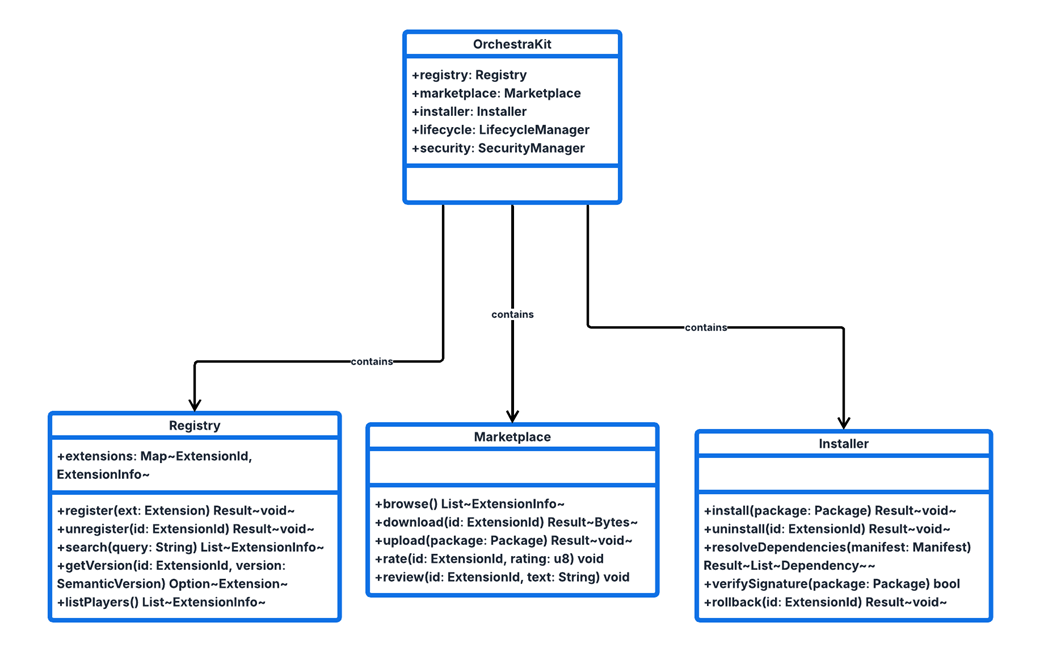
\includegraphics[width=1.15\textwidth]{images/diagrams/class_diagram/seperate_4_orchestra_kit_extension_ecosystem/Orchestra Kit Part1.png}
\caption{Orchestra Kit - Discovery and Distribution Components}
\label{fig:3.12-orchestra-discovery}
\end{figure}

\clearpage
\textbf{Component Group 2: Lifecycle and Security Management}

The second group manages extension lifecycle and security. The LifecycleManager implements the Chambering state machine, tracking extension states (Installed, Loading, Loaded, Activated, Running) and coordinating state transitions. The SecurityManager provides protection through sandboxing for process isolation, permission management for capability-based access control, and resource enforcement. The PermissionManager handles role-based access with permission checking, granting, revoking, and action auditing as illustrated in ~\ref{fig:3.13-orchestra-lifecycle}.

\begin{figure}[H]
\centering
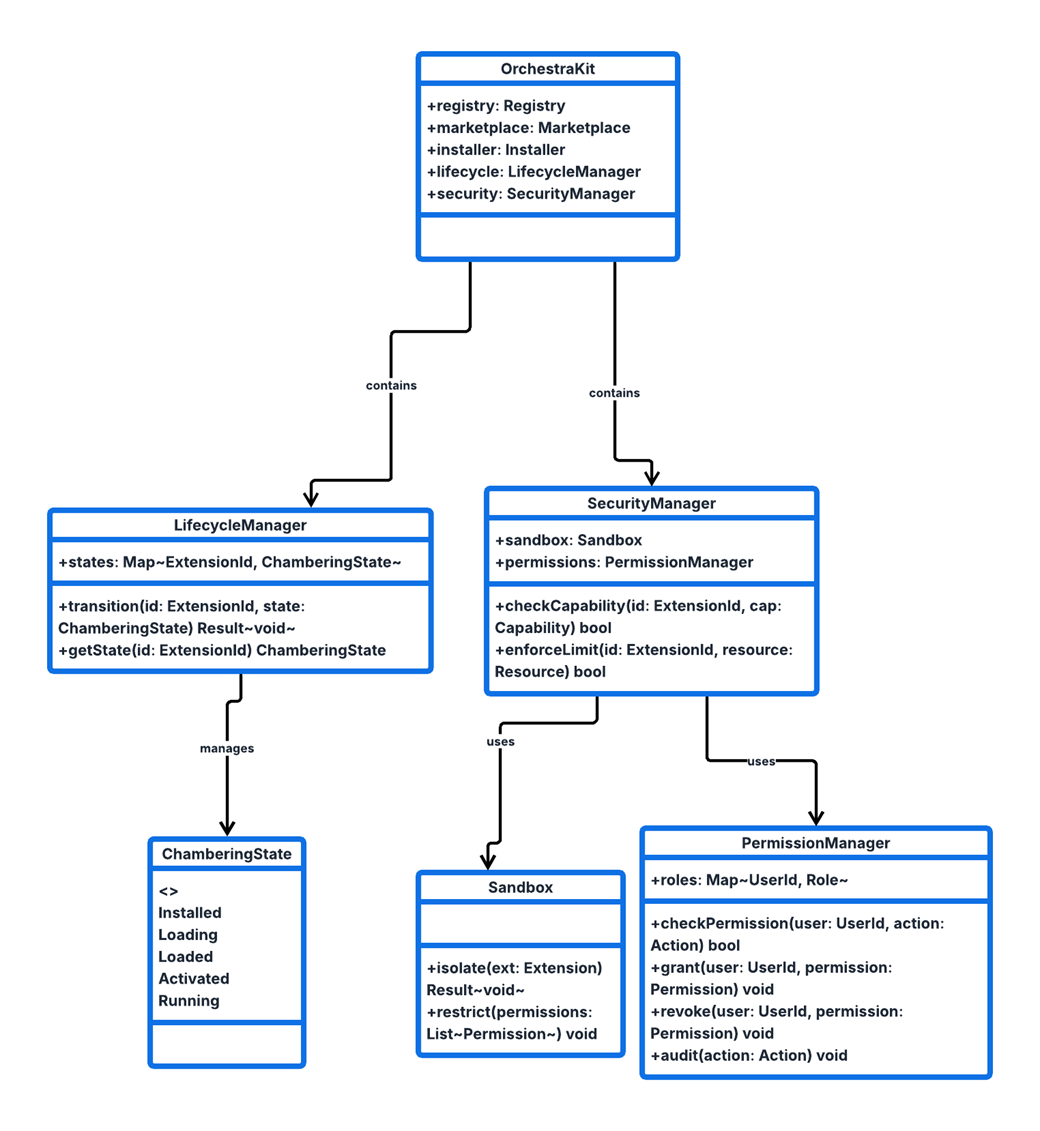
\includegraphics[width=1.15\textwidth]{images/diagrams/class_diagram/seperate_4_orchestra_kit_extension_ecosystem/Orchestra Kit Part2.png}
\caption{Orchestra Kit - Lifecycle and Security Management Components}
\label{fig:3.13-orchestra-lifecycle}
\end{figure}

\clearpage
\textbf{Component Group 3: Development Toolchain}

The third group provides the development toolchain. CaretsCli offers command-line interface for creating new extensions, running tests, publishing to marketplace, and scaffolding from templates. ExtensionSdk provides the development framework with core SDK functionality, testing framework with mocks and fixtures, and metrics collection for performance monitoring. This toolchain supports the complete development workflow from project creation through marketplace publication as illustrated in ~\ref{fig:3.14-orchestra-toolchain}.

\begin{figure}[H]
\centering
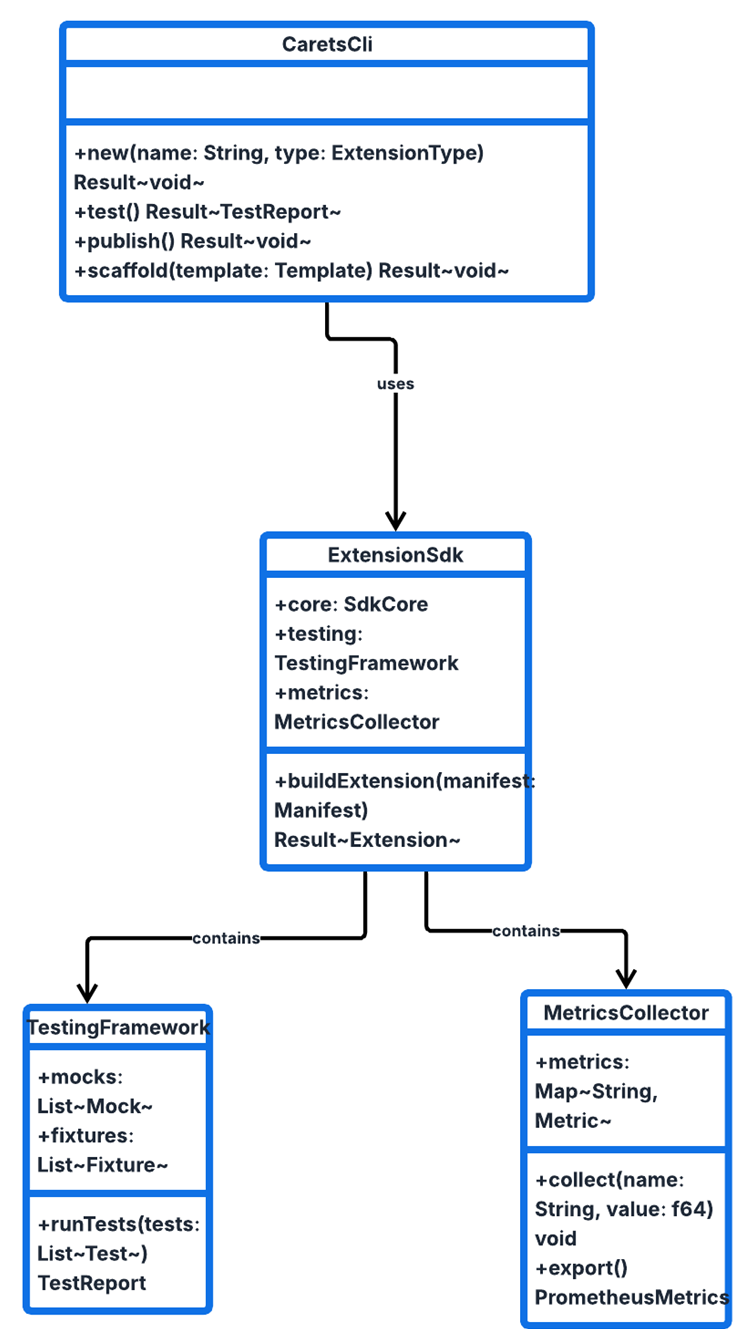
\includegraphics[width=0.95\textwidth]{images/diagrams/class_diagram/seperate_4_orchestra_kit_extension_ecosystem/CaretsCLISDK.png}
\caption{Orchestra Kit - Development Toolchain (Carets CLI and SDK)}
\label{fig:3.14-orchestra-toolchain}
\end{figure}


\subsection*{3.7.3 Extension Lifecycle and Chambering Process}

The extension lifecycle follows a well-defined state machine known as the Chambering process, governing transitions from installation through activation and execution. Extensions progress through distinct states including Installed, Loading, Loaded, Activating, Active, Deactivating, Unloading, and Uninstalled. Each state transition is carefully managed to ensure proper initialization before use and efficient resource management throughout the lifecycle.

The Chambering process ensures that extensions are properly validated before activation, resources are allocated efficiently during loading, and cleanup occurs systematically during unloading. State transitions are atomic operations that either complete successfully or roll back to the previous stable state, preventing partial initialization that could compromise system stability. The state machine governs all possible transitions and ensures that extensions follow the correct lifecycle path as illustrated in ~\ref{fig:3.15-extension-lifecycle}.

\begin{figure}[H]
\centering
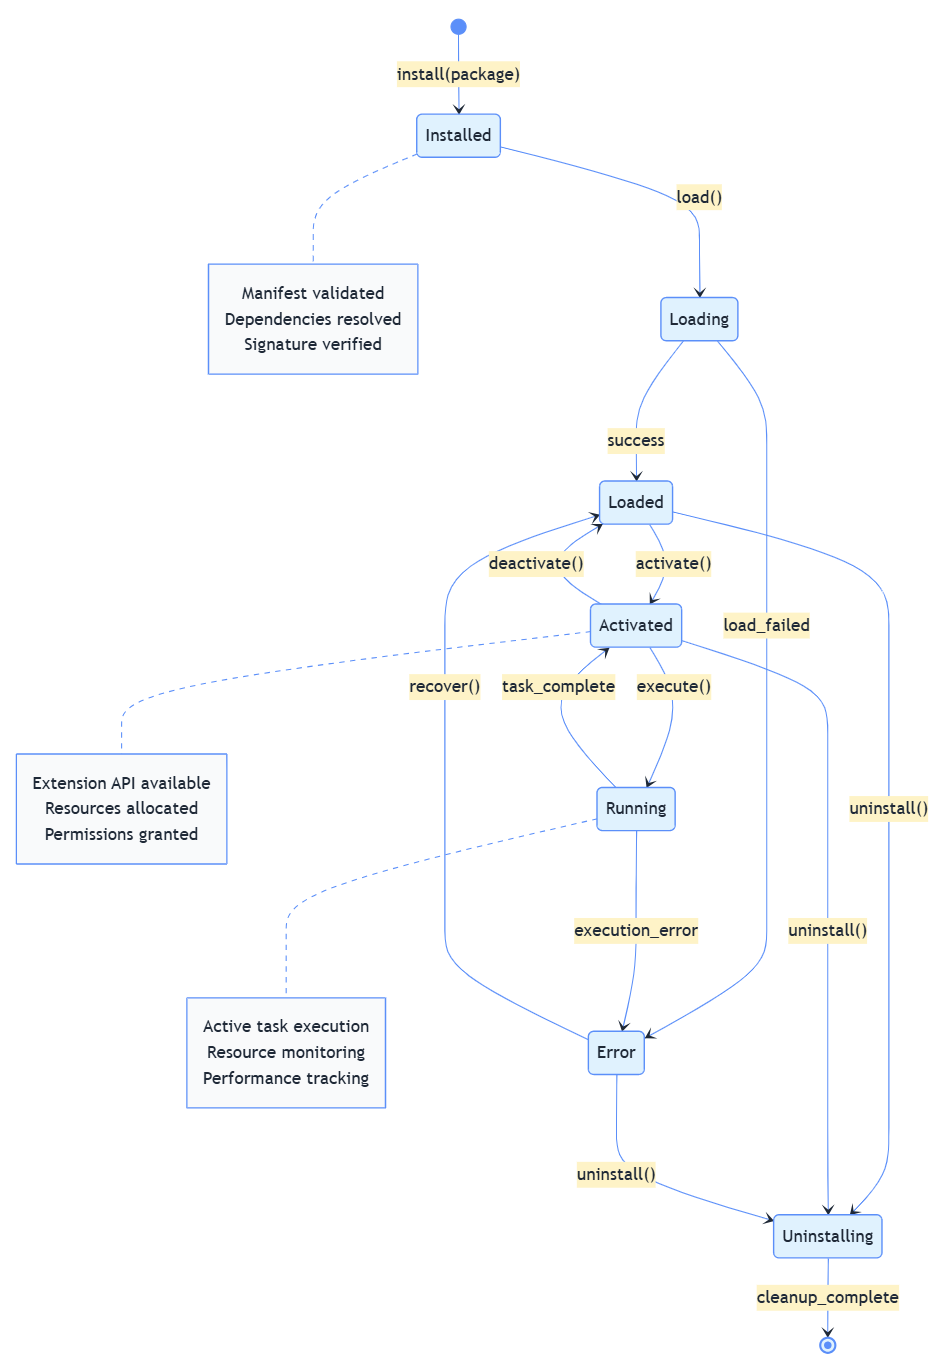
\includegraphics[width=1.05\textwidth]{images/diagrams/state_diagram/1_extension_lifecycle_chambering.png}
\caption{Extension Lifecycle State Machine}
\label{fig:3.15-extension-lifecycle}
\end{figure}

\subsection*{3.7.4 Extension Installation State Management}

The installation process manages eight distinct states ensuring reliable extension deployment with comprehensive security validation, dependency resolution, and automatic rollback capabilities:

\begin{compactlist}
    \item \textbf{Browsing}: User selection validation in marketplace
    \item \textbf{Downloading}: Network connectivity and package integrity verification
    \item \textbf{Verifying}: Signature validation and malware scanning
    \item \textbf{ResolvingDeps}: Semantic versioning and conflict detection with automatic dependency download
    \item \textbf{Installing}: File system operations and registration
    \item \textbf{Installed}: Successfully deployed and ready for loading
    \item \textbf{RollingBack}: State restoration and cleanup for failed installations
    \item \textbf{Failed}: Detailed error logging and reporting
\end{compactlist}

This state machine addresses critical deployment challenges including security validation through comprehensive signature verification and integrity checks, dependency resolution with automatic detection and conflict resolution, rollback capability for failed installations with complete state restoration, and seamless user experience with detailed progress feedback and error reporting.

\subsection*{3.7.5 Extension Development Workflow}

The extension development workflow provides comprehensive tooling support through the Carets command-line interface. The workflow encompasses the complete development lifecycle from initial project creation through marketplace publication. Developers begin by scaffolding new extension projects with proper structure and manifests, then implement functionality using the provided SDK and APIs. The workflow includes integrated testing frameworks for validation, security signing for package integrity, and automated publication to the marketplace.

The development process emphasizes several key aspects. Automated scaffolding generates complete project structures with proper manifests and configuration files. Integrated testing provides comprehensive frameworks that validate functionality before publication. Security validation through cryptographic signing and verification ensures package integrity and authenticity. Marketplace integration enables seamless publication with automated quality checks and version management. The complete workflow guides developers through each stage systematically as illustrated in ~\ref{fig:3.16-extension-development}.

\begin{figure}[H]
\centering
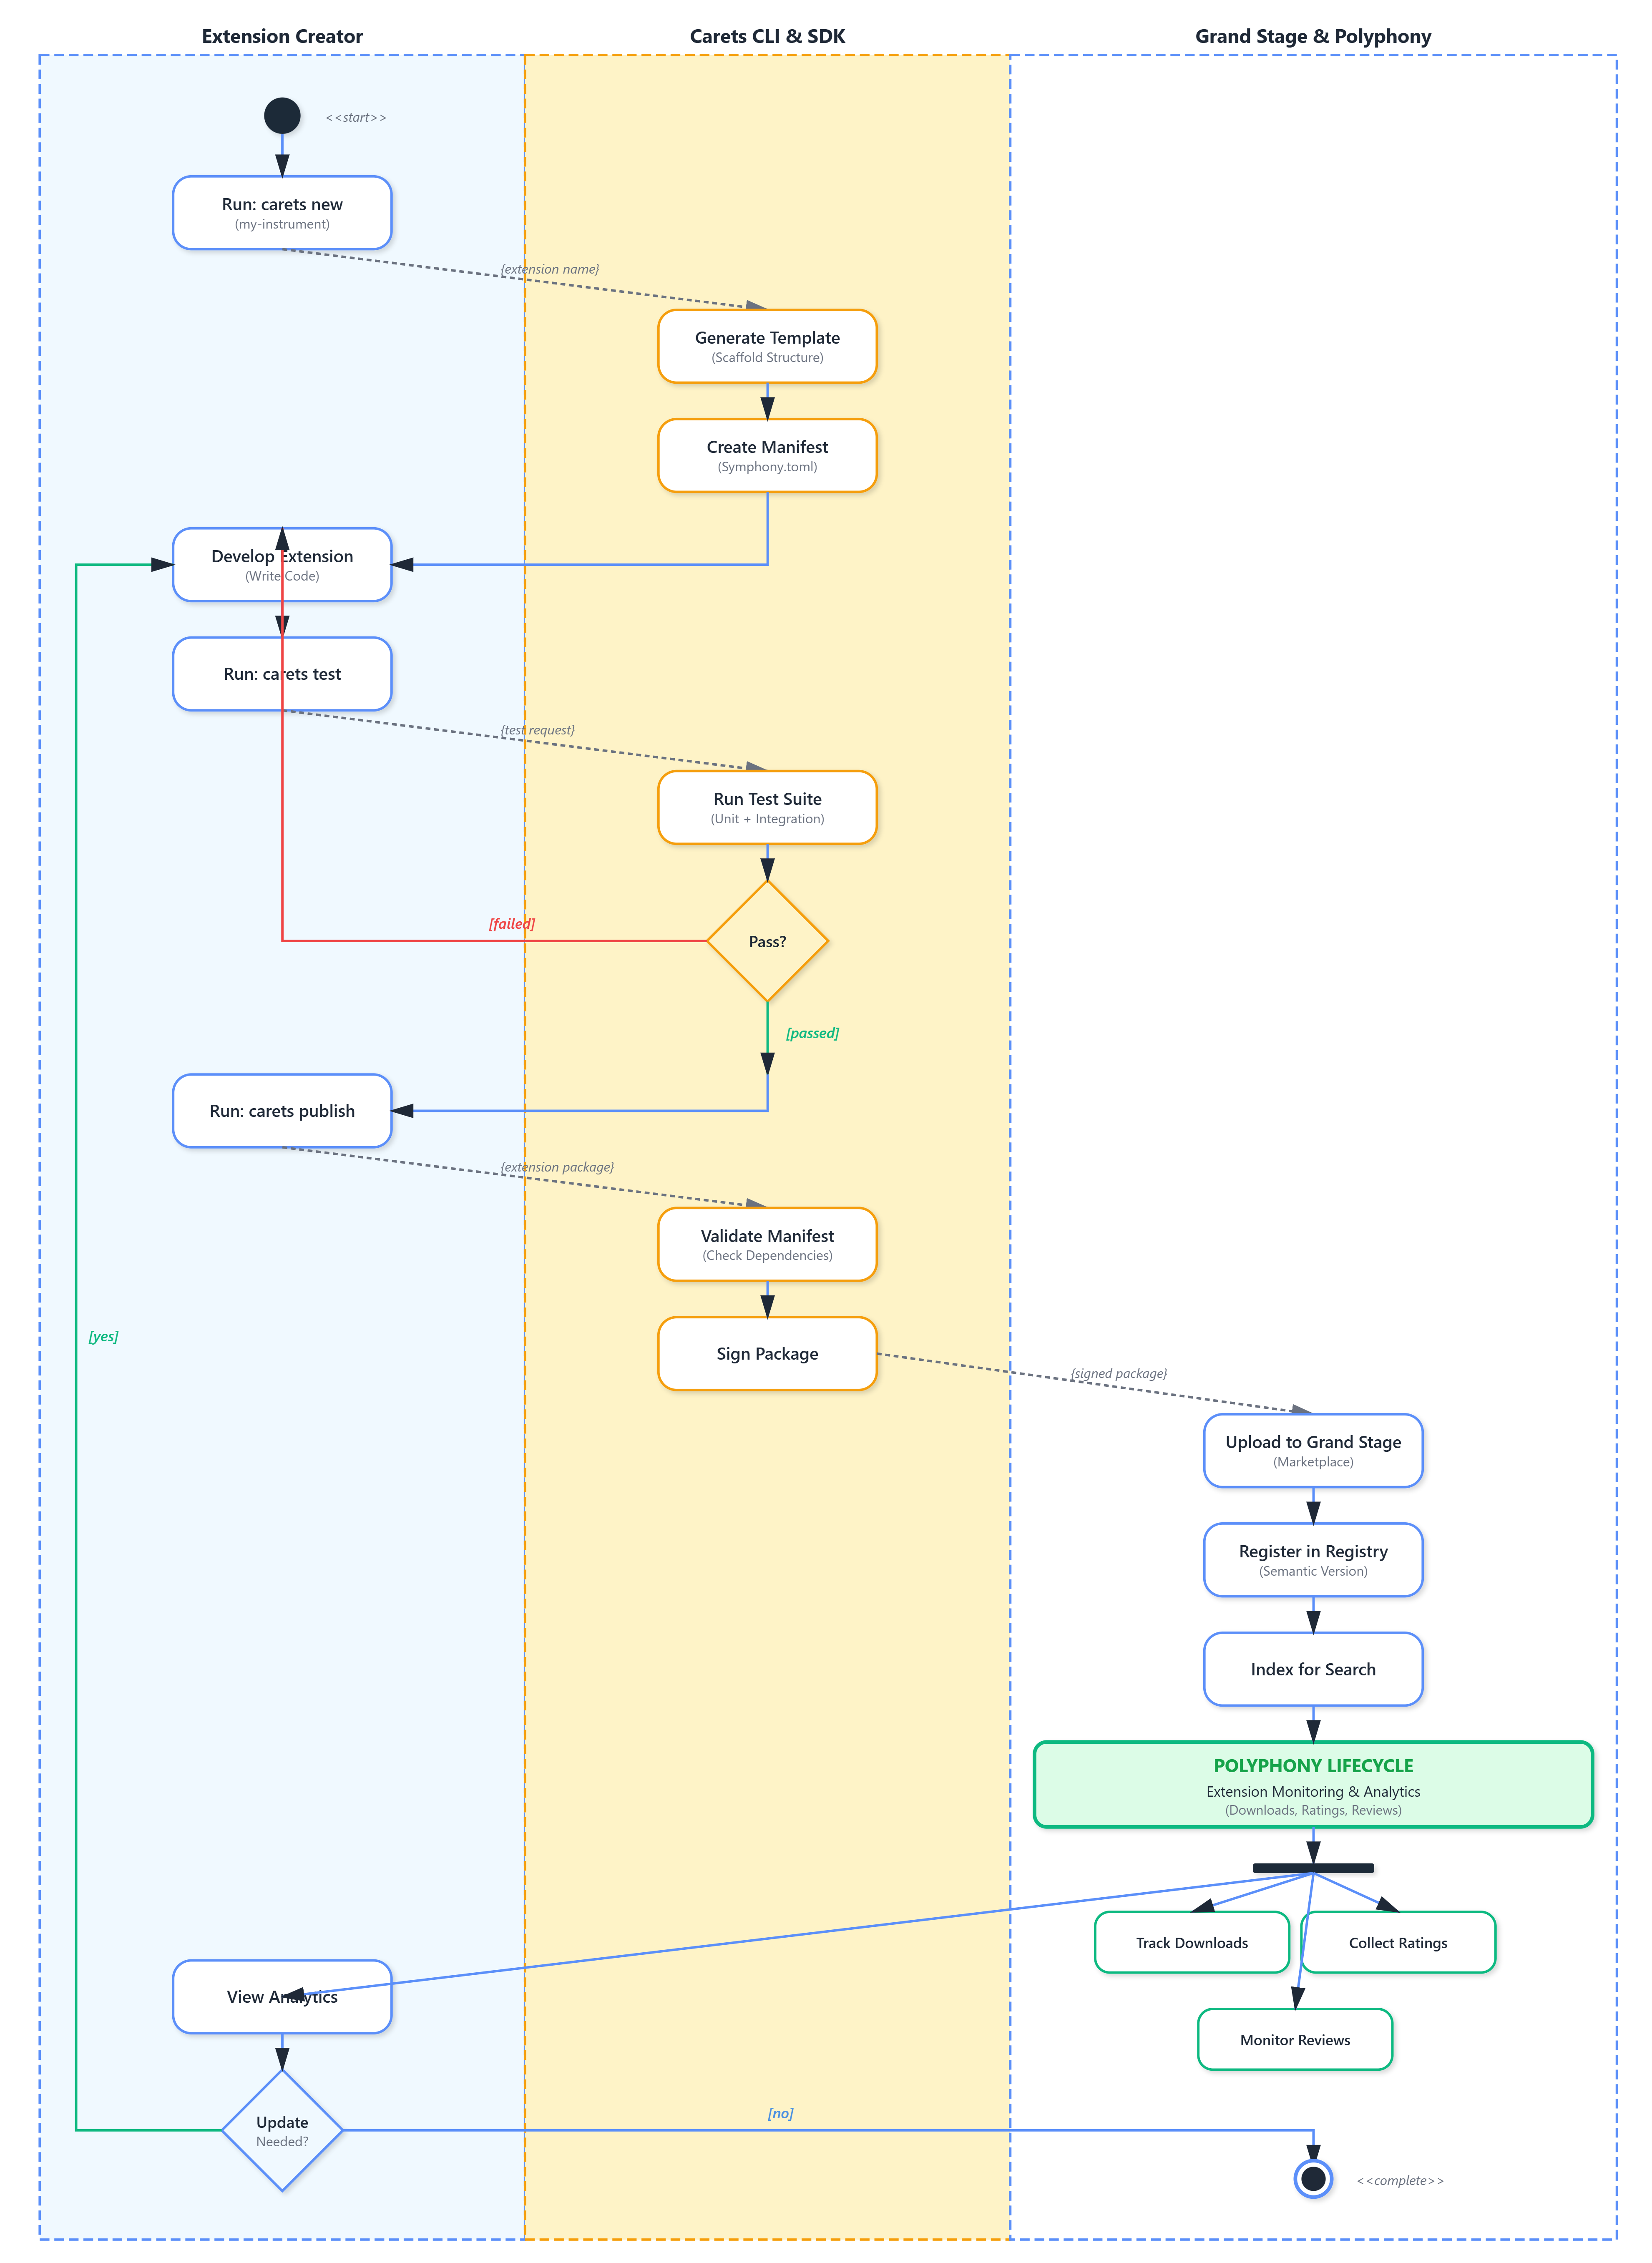
\includegraphics[width=1.15\textwidth]{images/diagrams/activity_diagram/symphony-extension-development.png}
\caption{Extension Development Workflow}
\label{fig:3.16-extension-development}
\end{figure}


% \subsection*{Marketplace and Ecosystem}

% The Grand Stage marketplace serves as the primary distribution channel for community and commercial extensions, implementing discovery through intelligent categorization and search capabilities, trust through comprehensive review processes and security scanning, quality through performance monitoring and user feedback, and sustainability through multiple monetization models supporting extension creator businesses.

% The marketplace supports multiple monetization strategies creating a sustainable ecosystem:

% \begin{compactlist}
%     \item \textbf{Free and Open Source}: Community-driven development and reputation building
%     \item \textbf{Freemium}: Basic functionality free with premium features available
%     \item \textbf{Usage-Based}: Pricing tied to actual consumption of resources or API calls
%     \item \textbf{Subscription}: Regular access fees for ongoing value delivery
%     \item \textbf{Enterprise Licensing}: Custom arrangements for organizational deployments
% \end{compactlist}

% Organizations can extend the public marketplace with private extension capabilities including internal-only extensions for proprietary workflows, role-based permissions for extension installation and usage, audit trails and governance controls for regulated environments, and professional services for specialized extension creation.
